\section{Durchführung}
\label{sec:Durchführung}

\subsection{Justage}

    Zunächst werden gemäß der Anleitung Startparameter eingestellt.
    Dann wird die Frequenz feinabgestimmt

    feinabstimmung damit keine schwingung mehr auftritt
    phase einstllen damit alles auf realteil liegt
    feldhomogenität maximieren, indem FID versucht wird zu maximieren 
    indem der Gradient eingestellt wird

    Pulslänge einstellen "A" und B"

    \begin{figure}[htbp]
        \centering
        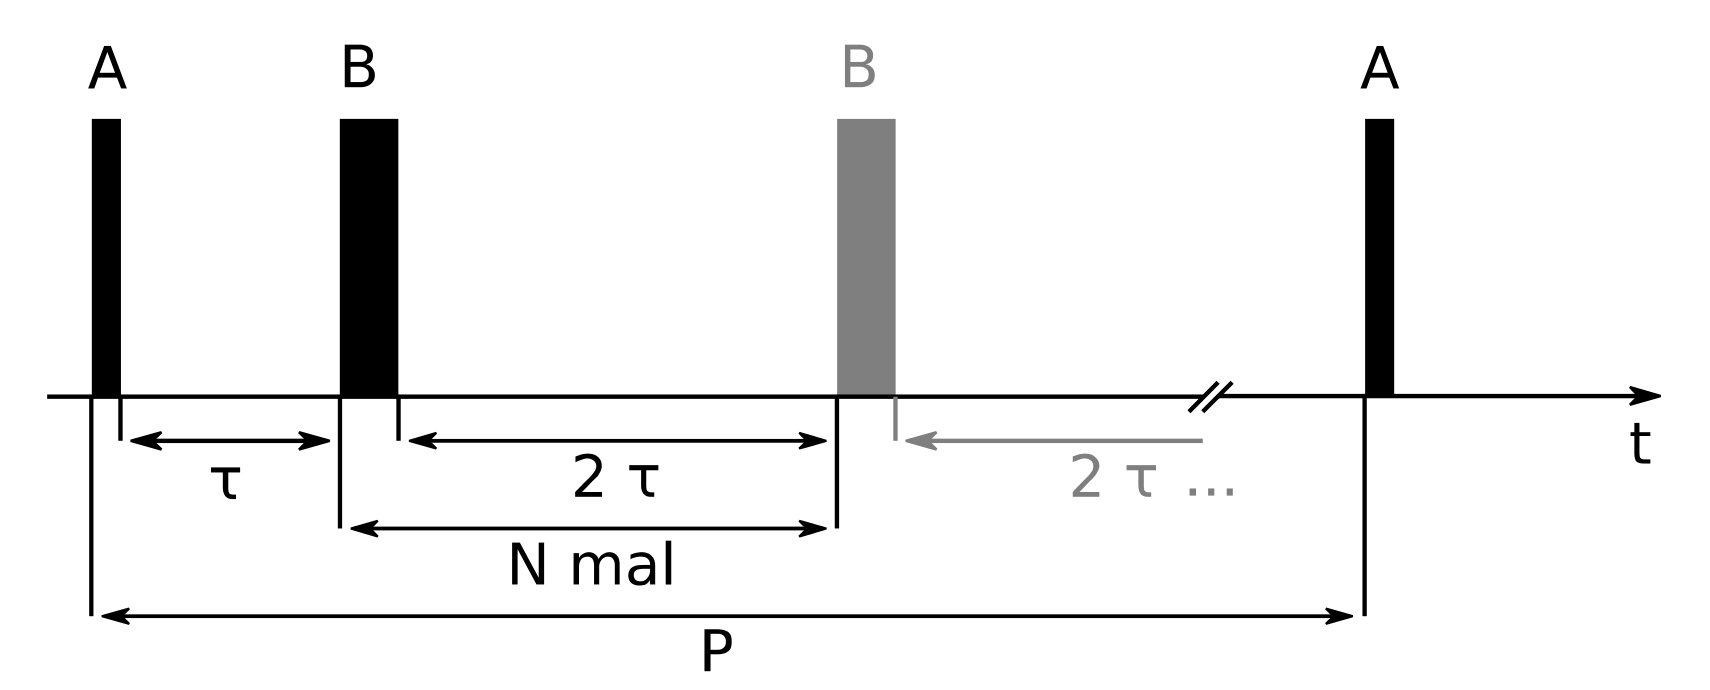
\includegraphics[width=\textwidth]{figures/pulsprogramm.png}
        \caption{<caption>}
        \label{<label>}
    \end{figure}

    

\subsection{}
\subsection{Justage}
\subsection{Justage}

